% ============================================================
% LATEX TEMPLATE FOR STUDY NOTES (ENGLISH)
% ============================================================
% General-purpose template for converting study notes
% (originally written in Markdown or in source code files)
% into a LaTeX document, for any book.
%
% Design philosophy: body text and cover in the standard LaTeX font (Computer
% Modern), no other font packages, no running header, no table of contents. The body follows
% the model of a classic technical book: plain text, footer with the
% page number only. The cover follows the model of a simple thesis
% title page: white paper, centered text, and a single small
% drawing (a transistor) as the only decoration.
%
% This is the English version. All visible text in the document is
% in English. The Portuguese version is the file template_pt-br.tex.
%
% Conversion instructions:
%
% - When converting notes from Markdown into this file, keep the
%   original language of the notes exactly as written.
% - Do not change, rewrite or translate the content of the notes.
%   Only format it properly for LaTeX (sections, code blocks,
%   emphasis, lists etc.).
% - Code comments are part of the notes and must also be kept in
%   the original language.
% - If the notes of the book are in Portuguese, use the Portuguese
%   version of the template (template_pt-br.tex), so that all
%   visible text (cover, credits, fixed titles) follows the language
%   of the notes.
%
% Usage:
%
% 1. Copy this file to start the notes for a new book.
% 2. Fill in the fields marked with <...> in the "document variables"
%    section below. It is the only place you need to edit to
%    configure the whole document.
% 3. If the book is not about programming, the listings package and
%    the code block can be removed.
% 4. Duplicate the section block for each chapter of notes.
% 5. Compile with pdflatex (twice, so cross-references come out
%    correct).

\documentclass[12pt,a4paper]{article}

% ============================================================
% Language and encoding
% ============================================================
\usepackage[utf8]{inputenc}
\usepackage[T1]{fontenc}
\usepackage[english]{babel}
\usepackage{lmodern} % Latin Modern: the standard vector version of Computer Modern

% ============================================================
% Page
% ============================================================
\usepackage{geometry}
\geometry{margin=2.5cm}
\usepackage[protrusion=true,expansion=true]{microtype}

% ============================================================
% Graphics and font used only on the cover. The cover uses the same
% font as the body (Computer Modern), as in a classic thesis title
% page. To use a different font on the cover only, edit the command
% below (for example, \fontfamily{bch}\selectfont for Charter,
% "ppl" for Palatino or "ptm" for Times).
% ============================================================
\usepackage{tikz}
\usetikzlibrary{arrows.meta}
\newcommand{\coverserif}{\rmfamily}
\usepackage{xcolor}
% Classic scheme: black ink on white paper, gray for secondary text.
\definecolor{coverfg}{HTML}{000000}    % black (strokes and main text)
\definecolor{coverdim}{HTML}{555555}   % dark gray (secondary text)

% ============================================================
% Lists
% ============================================================
\usepackage{enumitem}
\setlist{topsep=4pt,itemsep=2pt}

% ============================================================
% Footer: no header, only the page number.
% ============================================================
\usepackage{fancyhdr}
\pagestyle{fancy}
\fancyhf{}
\renewcommand{\headrulewidth}{0pt}
\renewcommand{\footrulewidth}{0pt}
\fancyfoot[C]{\footnotesize\thepage}

% ============================================================
% Code blocks: plain monospaced text, no frame, no background,
% no line numbers.
% ============================================================
\usepackage{listings}

% Replace "Scheme" with the language relevant to this book, or remove
% this definition and use \lstset{language=...} with a language
% already supported by listings (Python, C, Java etc.)
\lstdefinelanguage{Scheme}{
	morekeywords={},
	sensitive=true,
	morecomment=[l]{;},
}

\lstset{
	language=Scheme,
	basicstyle=\ttfamily\small,
	commentstyle=\ttfamily,
	frame=none,
	numbers=none,
	breaklines=true,
	showstringspaces=false,
	columns=fullflexible,
	xleftmargin=1.5em,
}

% Inline terms/definitions: term in bold followed by running text,
% no boxes and no color. Usage: \term{Definition} text...
\newcommand{\term}[1]{\textbf{#1.}}

% ============================================================
% Document variables: fill these in for each new book
% ============================================================
\newcommand{\bookTitle}{<BOOK TITLE>}
\newcommand{\bookShortTitle}{<SHORT TITLE OR ACRONYM>}
\newcommand{\bookAuthor}{<BOOK AUTHOR(S)>}
\newcommand{\studentName}{Miquéias Alves Medeiros}
\newcommand{\documentKeywords}{<KEYWORD1, KEYWORD2, KEYWORD3>}
% License: CC BY-NC-ND 4.0, the most restrictive of the Creative
% Commons licenses (SPDX identifier: CC-BY-NC-ND-4.0). Allows only
% reading and redistributing the unchanged work, with attribution.
\newcommand{\documentLicense}{This material is licensed under the Creative Commons Attribution-NonCommercial-NoDerivatives 4.0 International license (SPDX: CC-BY-NC-ND-4.0). Reading and full redistribution with attribution are permitted; commercial use and the creation of derivative works are prohibited. \url{https://creativecommons.org/licenses/by-nc-nd/4.0/}}

% Full bibliographic reference
\newcommand{\fullReference}{%
	<SURNAME>, <Name>. \textit{\bookTitle}. <edition>. <City>: <Publisher>, <year>.%
}

% ============================================================
% Hyperlinks and PDF metadata: links work, but stay invisible,
% as in a printed document.
% ============================================================
\usepackage[hidelinks]{hyperref}
\hypersetup{
	pdftitle={\bookTitle: Study notes},
	pdfauthor={\studentName},
	pdfsubject={Study notes on \bookTitle},
	pdfkeywords={\documentKeywords},
}

\begin{document}

% ============================================================
% Cover: simple thesis-style title page. White paper, everything
% centered, normal page margins. Top: type of document and title.
% Middle: a drawing of an abstract bipolar transistor (base,
% collector and emitter) in thin lines, surrounded by rings and
% connected to circuit traces, the only decoration.
% Bottom: author of the notes and date.
% ============================================================
\begin{titlepage}
	\thispagestyle{empty}
	\centering
	\coverserif
	\vspace*{1.5cm}

	{\small\bfseries\color{coverdim}\MakeUppercase{Study notes}\par}
	\vspace{0.4cm}
	{\color{coverfg}\rule{2cm}{0.6pt}\par}
	\vspace{1.0cm}

	{\bfseries\fontsize{24}{30}\selectfont\color{coverfg} \bookTitle\par}
	\vspace{0.8cm}
	{\normalsize\color{coverdim} Based on the work of \bookAuthor\par}

	\vfill

	% transistor drawing: concentric rings, envelope, base/collector/emitter,
	% parallel traces and square pads at the ends of the traces
	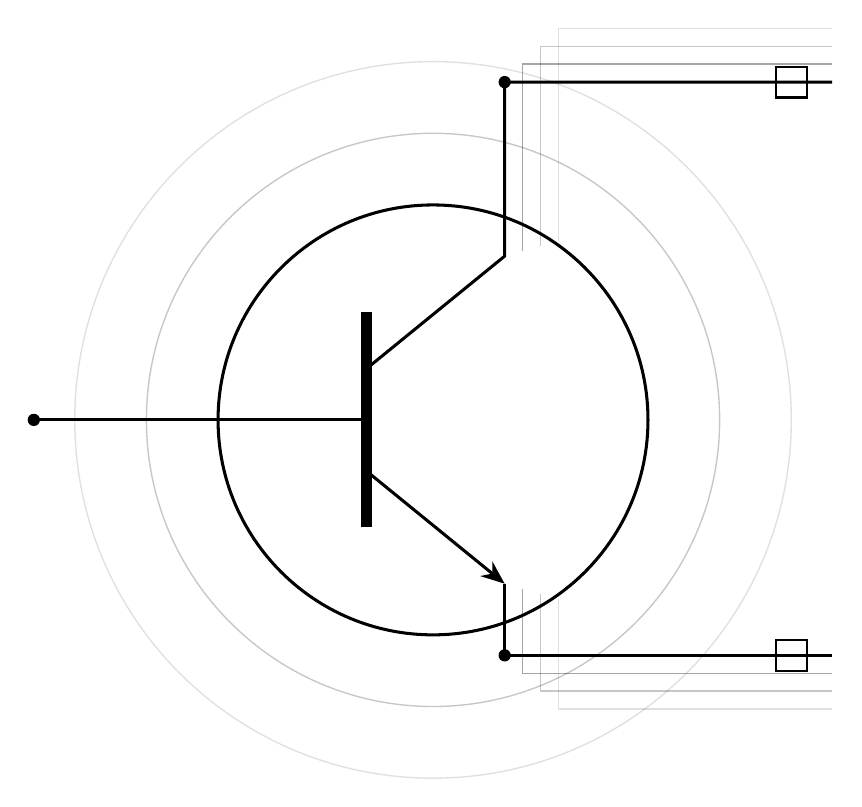
\begin{tikzpicture}[scale=0.65, coverfg]
		% subtle concentric rings
		\foreach \r/\o in {5.6/0.22,7.0/0.12} {
				\draw[draw opacity=\o, line width=0.5pt] (0,0) circle (\r);
			}

		% transistor envelope
		\draw[line width=1.1pt] (0,0) circle (4.2);

		% base: channel bar and terminal on the left
		\draw[line width=4pt] (-1.3,-2.1) -- (-1.3,2.1);
		\draw[line width=1.1pt] (-7.8,0) -- (-1.3,0);
		\fill (-7.8,0) circle (0.12);

		% collector: diagonal and trace that goes up and exits to the right
		\draw[line width=1.1pt] (-1.3,1.0) -- (1.4,3.2) -- (1.4,6.6) -- (7.8,6.6);
		\fill (1.4,6.6) circle (0.12);

		% emitter: diagonal with arrow and trace that goes down and exits to the right
		\draw[line width=1.1pt, -{Stealth[length=3mm,width=2.4mm]}]
		(-1.3,-1.0) -- (1.4,-3.2);
		\draw[line width=1.1pt] (1.4,-3.2) -- (1.4,-4.6) -- (7.8,-4.6);
		\fill (1.4,-4.6) circle (0.12);

		% thin parallel traces, echoing the collector and emitter routes
		\foreach \k/\o in {1/0.35,2/0.22,3/0.12} {
				\draw[draw opacity=\o, line width=0.5pt]
				(1.4+\k*0.35,3.2+\k*0.1) -- (1.4+\k*0.35,6.6+\k*0.35) -- (7.8,6.6+\k*0.35);
				\draw[draw opacity=\o, line width=0.5pt]
				(1.4+\k*0.35,-3.2-\k*0.1) -- (1.4+\k*0.35,-4.6-\k*0.35) -- (7.8,-4.6-\k*0.35);
			}

		% square pads at the ends of the traces
		\foreach \yy in {6.6,-4.6} {
				\draw[line width=0.8pt] (6.7,\yy-0.3) rectangle ++(0.6,0.6);
			}
	\end{tikzpicture}

	\vfill

	{\large\bfseries\color{coverfg} \studentName\par}
	\vspace{0.3cm}
	{\small\color{coverdim} \today\par}
	\vspace*{1cm}
\end{titlepage}

% ============================================================
% Credits page (back of the cover): the equivalent of the copyright
% page of a printed book, anchored to the bottom of the page.
% ============================================================
\thispagestyle{empty}
\vspace*{\fill}
\begin{flushleft}
	\footnotesize
	\bookTitle: Study notes\par
	\smallskip
	Based on the work of \bookAuthor.
	\par
	\smallskip
	Notes written by \studentName\ on \today.
	\par
	\smallskip
	\documentLicense
\end{flushleft}
\newpage

% ============================================================
% Dedication: a single sentence, vertically centered on the page
% and right-aligned.
% ============================================================
\thispagestyle{empty}
\vspace*{\fill}
\begin{flushright}
	\itshape I fight on the battlefield for those I love.
\end{flushright}
\vspace*{\fill}
\newpage

% ============================================================
% Content: duplicate the block below for each chapter
% ============================================================
\section{Notes on ch. <NUMBER>: <CHAPTER TITLE>, pp. <XX> to <XX>}

Introductory or explanatory text goes here.

\term{Definition} Use this convention for key concepts: the term
in bold, followed by running text, with no boxes or color highlights.

% Remove this block if not applicable to the book
\begin{lstlisting}
<example code here>
\end{lstlisting}

More explanatory text.

\newpage
% The thebibliography environment already inserts the "References"
% title (via \refname, translated by babel); do not add
% \section*{References}.
\begin{thebibliography}{9}

	\bibitem{reference1}
	\fullReference

\end{thebibliography}

\end{document}
